\documentclass[12pt,a4paper,bibliography=totocnumbered,listof=totocnumbered]{scrartcl}
\usepackage[ngerman]{babel}
\usepackage[utf8]{inputenc}
\usepackage{amsmath}
\usepackage{amsfonts}
\usepackage{amssymb}
\usepackage{graphicx}
\usepackage{fancyhdr}
\usepackage{tabularx}
\usepackage{geometry}
\usepackage{setspace}
\usepackage[right]{eurosym}
\usepackage[printonlyused]{acronym}
\usepackage{subfig}
\usepackage{floatflt}
\usepackage[usenames,dvipsnames]{color}
\usepackage{colortbl}
\usepackage{paralist}
\usepackage{array}
\usepackage{titlesec}
\usepackage{parskip}
\usepackage[right]{eurosym}
\usepackage{picins}
\usepackage[subfigure,titles]{tocloft}
\usepackage[pdfpagelabels=true]{hyperref}

\usepackage{listings}
\inputencoding{utf8}
\lstset{basicstyle=\footnotesize, captionpos=b, breaklines=true, showstringspaces=false, tabsize=2, frame=lines, numbers=left, numberstyle=\tiny, xleftmargin=2em, framexleftmargin=2em}
\makeatletter
\def\l@lstlisting#1#2{\@dottedtocline{1}{0em}{1em}{\hspace{1,5em} Lst. #1}{#2}}
\makeatother

\geometry{a4paper, top=27mm, left=30mm, right=20mm, bottom=35mm, headsep=10mm, footskip=12mm}

\hypersetup{unicode=false, pdftoolbar=true, pdfmenubar=true, pdffitwindow=false, pdfstartview={FitH},
	pdftitle={Lerntagebuch zu dem Cousera MOOC "Android Development"'},
	pdfauthor={Marco Seidler},
	pdfsubject={Independent Coursework 2},
	pdfcreator={\LaTeX\ with package \flqq hyperref\frqq},
	pdfproducer={pdfTeX \the\pdftexversion.\pdftexrevision},
	pdfkeywords={Independent Coursework 2},
	pdfnewwindow=true,
	colorlinks=true,linkcolor=black,citecolor=black,filecolor=magenta,urlcolor=black}
\pdfinfo{/CreationDate (D:20110620133321)}

\begin{document}

\titlespacing{\section}{0pt}{12pt plus 4pt minus 2pt}{-6pt plus 2pt minus 2pt}

% Kopf- und Fusszeile
\renewcommand{\sectionmark}[1]{\markright{#1}}
\renewcommand{\leftmark}{\rightmark}
\pagestyle{fancy}
\lhead{}
\chead{}
\rhead{\thesection\space\contentsname}
\lfoot{Lerntagebuch zu den Cousera MOOCs "'Android Development"}
\cfoot{}
\rfoot{\ \linebreak Seite \thepage}
\renewcommand{\headrulewidth}{0.4pt}
\renewcommand{\footrulewidth}{0.4pt}

% Vorspann
\renewcommand{\thesection}{\Roman{section}}
\renewcommand{\theHsection}{\Roman{section}}
\pagenumbering{Roman}

% ----------------------------------------------------------------------------------------------------------
% Titelseite
% ----------------------------------------------------------------------------------------------------------
\thispagestyle{empty}
\begin{center}
	
\includegraphics[scale=1]{Bilder/hs_os.jpg}\\
	\vspace*{2cm}
	\Large
	\textbf{Hochschule für Wirtschaft und Technik, Berlin}\\
	\vspace*{2cm}
	\Huge
	\textbf{Independent Coursework 2}\\
	\vspace*{0.5cm}
	\large
	über das Thema\\
	\vspace*{1cm}
	\textbf{Lerntagebuch zu den Cousera MOOCs "'Android Development"}\\
	\vspace*{2cm}
	
	\vfill
	\normalsize
	\newcolumntype{x}[1]{>{\raggedleft\arraybackslash\hspace{0pt}}p{#1}}
	\begin{tabular}{x{6cm}p{7.5cm}}
		\rule{0mm}{5ex}\textbf{Autor:} & Marco Seidler \\ 
		\rule{0mm}{5ex}\textbf{Matrikelnummer:} & 547431 \\ 
		\rule{0mm}{5ex}\textbf{Betreuerin:} & Prof. Dr. Debora Weber-Wulff \\ 
		\rule{0mm}{5ex}\textbf{Abgabedatum:} & 01.04.2015 \\ 
	\end{tabular} 
\end{center}
\pagebreak

% ----------------------------------------------------------------------------------------------------------
% Abstract
% ----------------------------------------------------------------------------------------------------------
\setcounter{page}{1}
\onehalfspacing
\titlespacing{\section}{0pt}{12pt plus 4pt minus 2pt}{2pt plus 2pt minus 2pt}
\rhead{KURZFASSUNG}
\section{Kurzfassung}
Dies ist mein Tagebuch über meine Erfahrung der zwei MOOCs zur Android Entwicklung, welche ich vom 18.02.2015 bis zum 18.03.2015 absolviert habe. \newline
Ich habe mich dabei sowohl für den Anfängerkurs als auch den Fortgeschrittenenkurs für Android Entwicklung eingeschrieben.    
Beide Kurse sind von Dr. Adam Porter von der Universität von Maryland angeboten und bauen aufeinander auf.\newline
Ich habe mich hierfür entschieden, da ich bereits im letzten Semester im Zuge des Praxisprojektes mit Android gearbeitet habe und bereits dort schon merkte, dass ich zwar gute Grundkenntnisse besitze, allerdings mir viel über konkrete Layout-fragen unbekannt ist. Besonders hilfreich wird mit vor allem der Fortgeschrittenenkurs sein. Wobei ich dennoch beide belegt habe, da diese aufeinander aufbauen. Allerdings finden diese dafür auch Zeitgleich statt.\newline
Das heißt ich belege im Zuge der Independent Coursework 2 den folgenden Anfängerkurs \textcolor[rgb]{0,0,1}{https://www.coursera.org/course/androidpart1} und den folgenden Fortgeschrittenenkurs \textcolor[rgb]{0,0,1}{https://www.coursera.org/course/androidpart2}.

\pagebreak

% ----------------------------------------------------------------------------------------------------------
% Verzeichnisse
% ----------------------------------------------------------------------------------------------------------
% TODO Typ vor Nummer
\renewcommand{\cfttabpresnum}{Tab. }
\renewcommand{\cftfigpresnum}{Abb. }
\settowidth{\cfttabnumwidth}{Abb. 10\quad}
\settowidth{\cftfignumwidth}{Abb. 10\quad}

\titlespacing{\section}{0pt}{12pt plus 4pt minus 2pt}{2pt plus 2pt minus 2pt}
\singlespacing
\rhead{INHALTSVERZEICHNIS}
\renewcommand{\contentsname}{II Inhaltsverzeichnis}
\phantomsection
\addcontentsline{toc}{section}{\texorpdfstring{II \hspace{0.35em}Inhaltsverzeichnis}{Inhaltsverzeichnis}}
\addtocounter{section}{1}
\tableofcontents
\pagebreak
\rhead{VERZEICHNISSE}
\listoffigures
\pagebreak
\listoftables
%\pagebreak
\renewcommand{\lstlistlistingname}{Listing-Verzeichnis}
{\labelsep2cm\lstlistoflistings}
\pagebreak

% ----------------------------------------------------------------------------------------------------------
% Abkürzungen
% ----------------------------------------------------------------------------------------------------------
\section{Abkürzungsverzeichnis}
\begin{acronym}[OSGi] % längste Abkürzung steht in eckigen Klammern
	\setlength{\itemsep}{-\parsep} % geringerer Zeilenabstand
	\acro{OSGi}{Open Service Gateway initiative}
\end{acronym}
\newpage

% ----------------------------------------------------------------------------------------------------------
% Inhalt
% ----------------------------------------------------------------------------------------------------------
% Abstände Überschrift
\titlespacing{\section}{0pt}{12pt plus 4pt minus 2pt}{-6pt plus 2pt minus 2pt}
\titlespacing{\subsection}{0pt}{12pt plus 4pt minus 2pt}{-6pt plus 2pt minus 2pt}
\titlespacing{\subsubsection}{0pt}{12pt plus 4pt minus 2pt}{-6pt plus 2pt minus 2pt}

% Kopfzeile
\renewcommand{\sectionmark}[1]{\markright{#1}}
\renewcommand{\subsectionmark}[1]{}
\renewcommand{\subsubsectionmark}[1]{}
\lhead{Kapitel \thesection}
\rhead{\rightmark}

\onehalfspacing
\renewcommand{\thesection}{\arabic{section}}
\renewcommand{\theHsection}{\arabic{section}}
\setcounter{section}{0}
\pagenumbering{arabic}
\setcounter{page}{1}

% ----------------------------------------------------------------------------------------------------------
% Einleitung
% ----------------------------------------------------------------------------------------------------------
\section{Einleitung}
Die folgenden Abschnitte sind alle nach dem gleichen Schema gestaltet. Wobei zunächst jeweils ein Ziel für die Woche gesetzt wird und eine Beschreibung des jeweiligen Tages. Am Ende jeder Woche folgt noch eine Zusammenfassung über erreichte Ziele und eine Auswertung der jeweiligen Woche. 

\subsection{Bilder}
Hier dargestellt die Cousera-Kurse in der Zusammenfassung auf dem Hauptauftritt \textcolor[rgb]{0,0,1}{https://www.coursera.org/}.  

\vspace{1em}
\begin{minipage}{\linewidth}
	\centering
	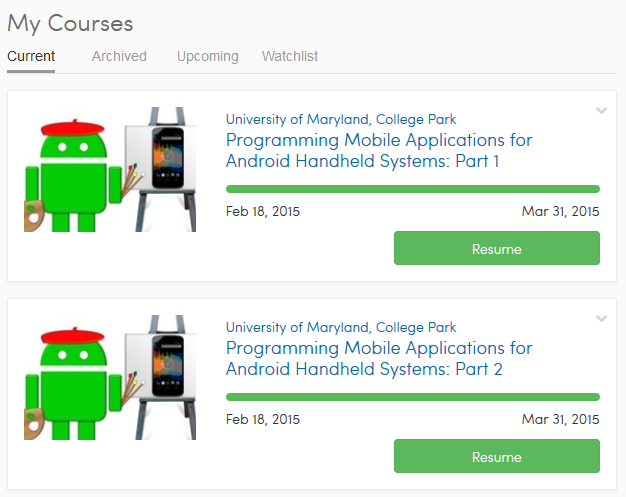
\includegraphics[width=0.7\linewidth]{Bilder/overview.png}
	\captionof{figure}[Darstellung der Cousera-Kurse]{Darstellung der Cousera-Kurse\footnotemark }
	\label{fig:osgi}
\end{minipage}
\footnotetext{Quelle: \url{https://www.coursera.org/}}

\pagebreak

% ----------------------------------------------------------------------------------------------------------
% Kapitel
% ----------------------------------------------------------------------------------------------------------
\section{Woche 0}

\subsection{Ziele für Woche 0}
Die Ziele für diese Woche sind recht wenige. Ein erstes hereinfinden in die Kurse und kennenlernen der Vorgehensweise stehen bei mir dabei im Mittelpunkt.

\subsection{Sonntag, 22. Februar 2015}
Ich habe heute damit begonnen die Videos zu betrachten um mich in die Kurse hineinzufinden. Ebenfalls habe ich eine kurze Vorstellung von mir in das Forum geschrieben, wobei hier Leute aus aller Welt teilzunehmen scheinen. 
Ich verwende parallel 2 Rechner, da die das Mitmachen - parallel zu den Videos - sehr vereinfacht.
Der Anfängerkurs fängt bei den Betriebssystemschichten von Android an und scheint wirklich sehr ausführlich zu sein. Das schließe ich basierend auf dem Wissen das ich über diese Thematik schon habe. 
Es kommen immer wieder kurze Fragen auf, die das gerade erzählt noch verstärken sollen. Die Fragen sind soweit ich das beurteilen kann gut gestellt und tragen wirklich zum Verständnis bei. Manchmal folgen auch mehrere hintereinander. Nach mehreren falschen Antworten wird einem die korrekte Antwort mitgeteilt, wobei mir auffällt, dass Dinge wie „was ist der IPC Binder Mechanism“ nicht nochmal erläutert werden, sondern nur als „die richtige Antwort“ dargestellt werden. Das finde ich etwas schade, da ich gerade bei so etwas die Zusatz Infos gebrauchen könnte.
Es war interessant zu erfahren, warum Android die Dalvik VM verwendet und nicht die normale JVM. Dies liegt daran, das Dalvik dafür ausgelegt ist in einem System zu laufen, was begrenzte Möglichkeiten hat. Dazu zählt der geringe CPU, weniger Ram und das geringe Batterieleben. 
Er gibt auch Hinweise in seinem Video, wo man zu einem bestimmten Topic mehr Informationen findet – in diesem Fall zur Dalvik VM. Er gibt auch Hinweise innerhalb der Fragen was ich sehr zuvorkommend finde. 
Er nutzt Android Emulator in seinem Video, was es sehr gut veranschaulicht was aktuell gemeint ist. Es gefällt mir sehr, dass er erläutert warum eine jeweilige Technik auf Android verwendet wird. Zum Beispiel das String System, das nur noch über den Operator R angesprochen wird in der Anwendung.
Er veranschaulicht gut wie verschiedene Activities in einander übergreifen, am Beispiel eines Music-Players. Interessant war auch von dem Location Manager zu hören, da wir das auch auf jeden Fall für das Praxisprojekt brauchen werden. 
Die Qualität des Tons variiert in den verschiedenen Videos. Das stört mich nicht sehr, aber es fällt auf. Die Videos scheinen älter zu sein, zum Einem da er nur kurz Android Studio erwähnt und zum anderem nur ältere Systeme empfiehlt. 
Er sagt, dass alle Emulatoren langsam sind. Das stimmt so nicht man kann sofern man Intel Kernel besitzt dem Emulator mit Hilfe des HAX Frameworks direkt auf der host CPU laufen lassen und muss nicht erst AMD Kerne emulieren, wodurch der Emulator signifikant schneller wird. Da der Tutor einen MAC verwendet fällt für ihn diese Option natürlich aus –weil keine Intel Kernel - aber das erwähnt er nicht einmal. 

\subsection{Reflektion Woche 0}
Es war ein interessanter Einstieg, ich bin gespannt wie sich die nächsten Wochen entwickeln werden. 
\pagebreak

% ----------------------------------------------------------------------------------------------------------
% Kapitel
% ----------------------------------------------------------------------------------------------------------
\section{Woche 1}

\subsection{Ziele der Woche 1}
Diese Woche habe ich das Ziel, dass ich die Videos und Übungen, welche Abgabetermin am 02.03.2015 soweit fertig stellen kann. Da ich die Woche zudem noch eine Erkältung bekommen habe, werde ich sehen, ob das realistisch ist.

\subsection{Dienstag, 24. Februar 2015}
Heute ist das erste Mal, dass ich den fortgeschrittenen Kurs besuche. Auch hier beginnt er auf einem sehr niedrigen Level – was ist ein Thread – allerdings erklärt er dieses dann auch sehr ausführlich. Er veranschaulicht es mit Bildern von mehreren CPUs. Aufgezeigt wird außerdem, wieso Nebenläufigkeit für manche Operationen wichtig ist. Ein Beispiel hierfür ist ein aufwendiges Fileloading. 
Parallel zu dem Video, habe ich die Samples von Github heruntergeladen und diese lokal auch selbst auf einem Emulator getested. Die Beispiele sind alle nicht in AndroidStudio erstellt, weshalb es recht lange dauert sie das erste Mal zu öffnen. 
Die Qualität der Fragen innerhalb der Video schwankt stark, manchmal sind diese nur vorhanden um sicherzustellen, dass man zugehört hat – offensichtliche Fragen – manchmal kommen jedoch auch Fragen auf, über welche man wirklich nachdenken muss. Das führt allerdings auch dazu, dass man wieder aufpasst. 
Man kann alle Folien herunterladen und abspeichern, was späteres Nachsehen vereinfacht.
Es fällt wieder auf, dass die Tonqualität stark innerhalb der Videos schwankt. Dafür wird sehr detailliert der Code erklärt, was ich sehr vorteilhaft finde, da es sehr zum Verständnis beiträgt. 
Interessant war die Info, dass jeder Thread einen eigenen Handler besitzt. Ich hatte etwas derartiges schon mal verwendet, wusste allerdings den Hintergrund dazu nicht (damals den Code einfach auf Stackoverflow gefunden). Auch das Prinzip des Loopers ist interessant – getMainloop() – habe ich schon mal verwendet, aber wie gesagt den Hintergrund dazu nicht gewusst. Manche Teile habe ich mehrfach angesehen, da ich nach einmaligem Sehen noch kein Verständnis aufgebaut hatte.
Über die Handlerklasse die erläutert wurde, müsste es an sich auch möglich sein die „Spring for Android“ Asynctasks aus dem Praxisprojekt auf Fertigstellung der Aufgabe testen zu können. Ich frage mich, ob dies wohl effektiver wäre als unser aktueller Aufbau mit dem Ottobus. dieser liefert eine ähnliche Funktionalität, ist dafür aber eine zusätzliche Abhängigkeit. 
Nun zum zweitem Teil – Networking. 
Inhalt hierfür werden Sockets, HttpURLConnection und der AndroidHttpClient sein. Ich bin gespannt, ob diese eine bessere Funktionalität als Spring bieten – Entity Mapping – aber ehrlich gesagt bezweifle ich das.  Anscheinend muss man bei der Verwendung von Sockets zum einem den Header selbst erstellen, als auch den Response der nur als String geliefert wird selber decodieren. Das ist eine sehr unschöne Vorgehensweise, zumindest empfinde ich dies so. Die HttpURLConnection Klasse verhält sich grundlegend genauso und gefällt mir damit ebenfalls nicht. 
Zum dem Quiz der Woche. 
Würde man versuchen das Zertifikat zu bekommen – ist mir die 90 Dollar nicht wert, da man Teil 1 und 2 gesondert braucht (2x 45 Dollar) – muss man sich um Betrug zu verhindern, mit der Webcam filmen lassen. Der Fakt gefällt mir nicht, da ich nicht weiß auf was sonst noch alles zugegriffen wird. Zudem ist es relativ leicht auch das zu fälschen. Virtuelle Webcam 10 Minuten Aufnahme von einem selbst beim Tippen und Nachdenken und dann das Ganze auf Endlosschleife in der Virtuellen Webcam abspielen. Ehrlich gesagt beugt das dem Betrügen  wenig bis überhaupt nicht vor.  Mit geringen Aufwand kann doch jeder beliebige Bekannte diesen Test für mich machen. 
Der Test selber setzt sich eigentlich nur aus den Fragen zusammen, welche auch schon während der Videos gesehen wurden. Wenn man diese dort beantwortet hat, kann man die Tests auch leicht bestehen. 
Nun werde ich zu dem Lab Teil übergehen, ich bin gespannt wie dieser sich gestaltet. Hier mache ich nur den aus dem Fortgeschrittenen Kurs, weil der aus dem Anfängerkurs ehr mit dem Aufsetzen der Umgebung zu tun hat. Wobei dieses dann auch noch veraltet ist und nicht einmal auf AndroidStudio basiert (was inzwischen schon Version 1.1 erreicht hat und damit nicht mehr im Alpha Stadium ist).
Die Lab beinhaltet eine PDF mit den Anweisungen, diese sehen auf den ersten Blick sehr ausführlich aus. Der Code soll als Zip Hochgeladen werden und damit automatisiert getestet werden. Ich vermute, dass dort nur geprüft wird, was die vordefinierten Tests machen und danach entschieden wird. 
Die Lab ist nach naherer Betrachtung ehr verwirrend als Lehrreich. Es wird zwar klar gesagt, was es leisten können soll, was soweit auch kein Problem ist. Kostete mich ca. 40 Minuten alles Wichtige umzusetzen. Allerdings soll von einer lokalen Datei Twitter Daten eingelesen werden. Diese Datei ist weder vorhanden, noch wird groß erläutert wo diese herkommen soll. Daher produziert mein AsyncTask nun bei jedem Ladeversuch eine Exception. Ich werde bei Gelegenheit mal in das Forum sehen, ob ich dort noch Infos bekomme zu der Abgabe. 

\subsection{Donnerstag, 26. Februar 2015}
Heute sind die neuen Kurse und Aufgaben freigegeben worden. Ich hatte die von Fortgeschrittenenkurs eigentlich erst zu 18:30 erwartet, dass ich als UTC-5 12.01 pm verstanden hatte aber anscheinend hält sich der Tutor nicht an diese Zeitangabe.
Ich habe meine Abgabe der ersten Aufgabe fertiggemacht, es ist unklar inwiefern sie richtig ist. Bei mir lokal schlägt sie fehlt, da keine Daten existieren die geladen werden können und ich auch keine Idee habe wo diese herkommen sollten. Die vorhandenen Helper-methode produzieren also einen Fehler. Damit ist aber dennoch auf jeden Fall erstmal die Abgaben der ersten Woche abgeschlossen und ich wende mich nun der neuen Aufgabe im Anfängerkurs zu.
Ich bearbeite alle Themen des Anfängerkurses, auch wenn mir diese Dinge vermutlich das meiste schon bekannt sein dürften, aber nur um sicher zu gehen. 
Zwischenzeitlich kam eine Motivation des Tutors für die Kurse in Form einer E-Mail wo er sich über die zahlreiche Teilnahme bedankte.
Nun zu den Videos des Anfängerkurses dieser Woche.
Er beginnt auf einem guten allgemeinen Level, was die Zusammenhänge aufzeigen soll. 
Erneut sind seine Beispielprojekte in einem sehr altem Stand Android 2.2 wobei der aktuelle Stand 5.1 ist. Im Video fordert er dazu auf das Beispielprojekt runterzuladen und parallel anzusehen. Nun für mich ist das kein Problem, da ich 2 PCs gleichzeitig verwende aber ansonsten müsste man an dieser Stelle das Video abbrechen und zu einem späteren Zeitpunkt fortsetzen, wobei sich nicht gemerkt wird an welcher Stelle im Video man gewesen ist. Im Video war nun ein Beispiel wo er auf eine Klasse im Code anspielt, welche eine Abstract Klasse überschreibt. Diese war allerdings nur über die Volltextsuche aufzufinden, da er nicht sagte in welchem Projekt, bzw. das genannte Projekt nicht existierte und anders hieß. 
Zu den Inhalten.
Die vier fundamentalen Komponenten waren interessant ContentProvider, Activity, BroadcastReceiver und Service. Wobei Activity die einzige Komponente ist, welche ein UI anbietet. Er erläutert gut wie man denselben source code für verschiedene Sprachen nutzen kann. Dafür muss man bei den String Definitionen nur dem Drüberlegenden Ordner mit dem Länder Präfix benennen - „String-it“ für Italienisch zum Beispiel. 
Auch die Infos zu mehreren Layouts sind sehr interessant, hier kann man angeben, wie sich das Layout auf verschiedenen Geräten verhalten soll. 
Sehr gut ist ebenfalls, dass gute Informationen vermittelt werden, über das Überschreiben der onCreate Methode in der MainActivity – das ist der Startpunkt der App – detaillierte Beschreibung was dort warum abläuft. Gefällt mir sehr gut diese Vorgehensweise. 
Der Anfängerkurs ist nicht ganz was ich erwartet hatte, es ist viel detaillierter und beschreibt mehr die Funktionen der einzelnen Codefragmente anstatt primitives Erstellen einer „Hallo Welt“ App. Gefällt mir sehr gut die Grundlagen auf diese Weise vermittelt zu bekommen. Es frischt mein bisher was ausschließliches Bücherwissen gut auf. 
Der Zweite Teil dreht sich um die Activity Class, ich bin gespannt was da an neuen Infos herauskommen wird. Der Activity Lifecycle (onCreate -> onStart -> onResume -> onPause -> onStop -> onDestroy) trägt wirklich gut zum Verständnis bei. So tiefgehend hatte ich mir das noch gar nicht angesehen. 
Eine gute Info war, dass man aufgrund des lifecycles und der Möglichkeit von Android bei „low memory“ Applikationen einfachen zu „killen“, ohne die onDestroy Methode aufzurufen und daher wichtige Aktionen – wie speichern - bei der onPause Methode ausführen sollte. Kann man auch als ein Final ansehen wie bei einem „Try Catch“ Block wie es scheint. Nun kommt er zu dem Teil der auch mir schon bekannt ist – das Intent-System von Android – HAX Beschleunigung. Diese Thematik kommt in meinen Augen recht spät. War aber auch ehr eine nette Zusammenfassung, daher nichts Neues für mich. 
Nun gehe ich zu dem wöchentlichen Quiz des Kurses über. Zum Beantworten musste man sogar relativ viel nachdenken, finde ich gut. Allerdings wird nicht überall gesagt, was die richtige Antwort ist das ich schade finde, weil es mir an manchen Stellen noch immer unklar ist. 
Nun zum Praktischen Teil und da er seine Sourcen mit Eclipse erstellt hat und ohne Gradle muss ich jedes Mal alle Projekte in diese Form setzen und das verursacht einen gewaltigen Konfigurationsaufwand. 
Aber dank Stackoverflow habe ich es dennoch anbekommen. Es kostete micht etwa 30 Minuten Aufwand bis ich die Lab lauffähig bekommen hatte.  Also viel Zeitaufwand bevor die eigentliche Aufgabe begonnen werden konnte. 
Die Übung an sich war lehrreich und unterhaltsam, also sehr gut gemacht und ist ebenfalls lauffähig auf meinem Emulator dank Gradle. 
Nach Abschluss kann ich sagen, es war doch eine lehrreiche Übung über den Activity Lifecycle. 

\subsection{Samstag, 28. Februar 2015}
Heute werde ich mich mit dem fortgeschrittenen Kurs für diese Woche beschäftigen. Thematik für heute sind User Notifikation, der BroadcastReceiver, sowie Alarms. Ich bin gespannt was dort so Neues vorgestellt wird. 
Zunächst geht es um Notifikations. 
Er beginnt dabei wieder mit dem Grund warum man diese Technologien gebrauchen kann. Das erste ist dabei der Toast, was sowas wie ein kurzer aufpoppender Text ist. Dieser ist mir schon bekannt, aber ich bin gespannt ob ich noch neue Infos dabei bekommen kann. Der „Custom View“ Teil war mir neu. Es ist gut dass immer noch Sachen dazukommen, die mir nicht bekannt sind. 
Auch die anderen Typen hat er jeweils erläutert, wozu man diese verwenden kann und wie man diese im Code verwendet. Diese Vorgehensweise finde ich sehr gut, da sie das Verständnis doch stark verbessert.
Nun zur zweiten Thematik dem Broadcast Receiver. 
Die Broadcast Klasse scheint an sich wie ein Observer-Pattern zu funktionieren, wobei sich ein Broadcast für einen Service registriert und dann auf ein Event das ausgelöst wird reagiert. 
Auch der Teil über den Broadcast war sehr detailliert und gut gemacht. Wichtig für mich war die Information, dass ein BroadcastReceiver nicht asynchron mit der Aufrufenden Operation kommunizieren kann. Der große Vorteil ist hierbei halt, dass man mit mehreren Empfängern arbeiten kann. Wobei man hier auch die Reihenfolge festlegen kann. Nun erinnert mich das Prinzip noch mehr an das Observer Pattern, da auch hier die Observable nicht mehr von den Observern angesprochen werden können. Anwendungen können über Broadcasts den aktuellen Akkustatus des Gerätes erfahren. So werden aufwendige Operationen bei einer geringen Restkapazität gar nicht erst gestartet. 
Nun zur letzten Thematik den Alarmen.
Alarms sind für bestimmte Zeitpunkte definierbar, diese können dabei einmal sein, oder beliebig oft wiederholt werden in einem bestimmten Intervall. Ähnlich wie der Windows Task Scheduler. Die unterschiedlichen Alarmtypen und wie diese sich verhalten zu sehen war recht interessant. 

So nun noch das Quiz zu den gerade durchgenommenen Themen, den Praxisteil werde ich an einen anderen Tag in Angriff nehmen. 
Die Fragen waren diesmal sogar recht anspruchsvoll und ich schaffte es auf Anhieb (erster Versuch) auch nur 54\% richtig zu beantworten. 

\subsection{Reflektion Woche 1 }
Es war eine interessante Woche, ich habe relativ viel gelernt. Mein Ziel habe ich leider nicht ganz geschafft, aber den praktischen Teil werde ich einfach nächste Woche bearbeiten zusammen mit den neuen Themen. Bisher werden aber viele Sachen angesprochen, die mir so noch nicht bekannt waren und mir durchaus irgendwann helfen könnten. 

\pagebreak

% ----------------------------------------------------------------------------------------------------------
% Kapitel
% ----------------------------------------------------------------------------------------------------------
\section{Woche 2}

\subsection{Ziele für Woche 2 }
Diese Woche möchte ich auf jeden Fall den praktischen Rest der letzte Woche noch erledigen und bin gespannt auf die neuen Teile, welche aber Mittwoch freigeschaltet werden. 

\subsection{Dienstag, 3. März 2015}
Heute beschäftige ich mich mit dem Praktischen Teil des fortgeschrittenen MOOC Woche 2.
Es ist wieder ähnlich aufgebaut wie die Aufgaben der letzten Male und nutzt auch wieder Twitter Daten um Informationen zu generieren. Wieder einmal ist das erste was geschieht das nach dem Laden des Projektes die Struktur dieses komplett kaputt ist und so nicht verwendbar. Es muss es wieder die Projektstruktur und Manifest geändert werden, damit die MainActivity gefunden werden kann. Ich nehme an das ist auf das Alter der Lab zurückzuführen und das kein Gradle verwendet wird. 
Wieder einmal ist das Hauptproblem beim Richten der Struktur nicht das eigentliche Einstellen, sondern das Finden der richtigen Punkte in Android Studio. Die Konfiguration funktioniert mal wieder überhaupt nicht und nervt zutiefst. Anscheinend hängt das damit zusammen, dass der Tutor das völlig veraltete Eclipse ADT verwendet und Android Studio eine gänzlich andere Projekt Struktur benötigt. Was nun dazu führt, das Dateien die genau an der Stelle liegen wo sie liegen sollen dennoch nicht gefunden werden können. Zumindest lerne ich langsam Projekte schneller neu zu konfigurieren, das ist auch etwas. Dieses Mal gelang es mit etwas schneller. Ich bin immer noch unsicher, was diesmal anders war, aber nachdem ich in die AndroidStudio Konfiguration geändert hatte, manuell das Kompilierte meines aktuellen Projektes löschte und Android Studio damit zwang das neu zu generieren, ging es direkt. 
Die Programmieraufgaben sind wieder gut gemacht, es steht da was gemacht werden muss – gekennzeichnet mit @TODO - und man muss es selber schreiben, was mit Hilfe von Google aber schnell gemacht ist. Dennoch ist das ganze sehr lehrreich. 
Soweit habe ich die Übung geschafft, auch wenn es doch recht aufwendig war, da immer wieder wichtige Infos fehlten, die einem erst später die Laufzeitumgebung mitgeteilt hat. 

\subsection{Donnerstag, 5. März 2015}
Heute befasse ich mich mit der dritten Woche der Android MOOCs. Ich beginne dabei genauso wie letzte Woche zunächst mit dem Anfängerkurs und setzte zu einem späteren Zeitpunkt im Fortgeschrittenenkurs daran an.
Als erstes fällt mir auf, dass im Gegensatz zu den letzten Labs diesmal gleich 3 Projekte den Praxisteil der Woche ausmachen. Es geht um Intents, Permissions und Fragments also an sich Dinge dir mir schon bekannt sind, aber die Informationen der letzten Wochen waren trotz meines Vorwissens auch sehr interessant also bin ich guter Dinge. 
Das erste Thema ist über Intents. Er  beginnt wieder damit zu erläutern, was für einen Zweck die Intent Klasse erfüllt und wie man diese einsetzt. Die Erläuterung, wie man einen Intent definieren und unterscheiden kann über eine Konstante, ist gut beschrieben. 
Die erste Frage, welche in das erste Video eingebaut ist, wurde viel zu spät aufgerufen und hat den Tutor damit im Satz unterbrochen und wirkte nicht sehr professionell. Die zweite Frage ist eine Definitionsfrage und zwingt einen das Video zu schließen sich zu merken, wo man war um die genannte Seite zu öffnen. Ich habe also geraten und die Frage direkt korrekt beantwortet – Glück gehabt. Nun erläutert er was die Antwortmöglichkeiten alle für einen Sinn gehabt haben. Na ja gut zu wissen wofür die einzelnen Dinge da sind. 
Auch im zweitem Video ist die erste Frage wieder nur beantworten, wenn man das Video schließt. 
Ich habe inzwischen einen zweiten PC dazu genommen und schaue dort nach ohne das Video zu schließen. 
Die Informationen über den Intentfilter waren sehr interessant – man muss eine Activity im Manifest definieren, damit sie gefunden wird. Macht man das nicht, wird ein Fehler geworfen. Allerdings erst zur Laufzeit was das ganze etwas nervig macht. Google Maps kann mit Intents umgehen, welche eine Action von 
\glqq intent.action\_view \grqq und ein Datenfeld mit den Geo-Schemata haben. 
Ein Fakt zu den Videos stört mich etwas. Die Untertitel scheinen von Hand geschrieben worden zu sein, zumindest sind mir mittlerweile mehrere Rechtschreibfehler aufgefallen. Erneut unterbricht ihn die Frage mitten im Satz. Es gab einen Versuch die Leute zu motivieren etwas in das Forum zu schreiben. Allerdings kam dieser Aufruf zum Einem als Frage und zum Anderem wieder so, dass er mitten im Satz unterbrochen wurde. Mir zudem gerade auf, dass diese Woche Optionale Inhalte besitzt – 1 zusätzliches Video. Die Qualität der Videos scheint stark zu variieren. 
Nun komme ich zur nächsten Thematik dieser Woche, den Permissions. 
Permission Probleme treten meiner Erfahrung auch nur zur Laufzeit auf. Auch diese müssen wie neue Intents im Manifest eingetragen werden. 
Er stellt eine Frage zu einem Sachverhalt, welchen er erst nach der Frage das erste Mal erwähnt! Gefällt mir gar nicht, dass die Fragen anscheinend so willkürlich auftauchen. Der Aspekt mit eigenen Permissions erstellen ist mir neu, scheint aber recht nützlich zu sein. 

Nun zum letzten offiziellen Teil. Ich habe vor mir auch das optionale Video anzusehen. 
Der letzte Teil befasst sich mit Fragments, ich habe mit diesen schon zu tun gehabt, besitze aber kein tiefgehendes Wissen dafür und bin daher gespannt was der Inhalt sein wird. 
Er zeigt zunächst wie man Fragmente einsetzen kann, um auf verschiedene Bildschirmgrößen verschiedene Layouts einzubinden (Smartphone und Tablet). Fragmente werden von Activities gehosted.  Fragmente haben einen anderen Lifecycle als Activities. So wird das Layout dort nicht bei onCreate erstellt, sondern erst bei onCreateView, was später aufgerufen wird, und das Fragment wird zur beinhaltenden Activity als View hinzugefügt. Interessant ist der Fakt, dass man Fragments auch dynamisch einer Activity, mit Hilfe des FragmentManagers, hinzufügen kann. Diese muss also nicht hardcodiert vorher schon festgelegt sein. 

Der optionale Teil beinhaltet das Registrieren im Amazon Appstore als Developer und wie man seine App dort anbietet. Amazon bietet auch eine kostenloses ebook an. Wobei für mich das ehr den Eindruck erweckt, als wollte man neue Kunden für Amazon binden, vielleicht hat Amazon etwas gespendet für die MOOC Erstellung und das war die Bedingung? Den Playstore erwähnt er gar nicht erst. Ich vermute ein Bezahlen des ebooks mit persönlichen Daten. Der zweite Teil ging um die Vorstellung eines Nebenläufigkeits MOOCs für Android. 
Nun komme ich zu dem Quiz für diese Woche.
Das Quiz war diesmal recht anspruchsvoll, habe es auf Anhieb nur auf 59\% gebracht. Leider ist am Ende noch immer unklar, warum manche Antworten falsch sind. Man bekam keine Lösung, oder Erklärung am Ende.
Gut nun komme ich zu dem letzten Teil für Heute – die Labs. Beginnen werde ich hier mit den Intents und hoffe, dass ich es inzwischen ein bisschen schneller hinbekomme die Projektstruktur einzurichten. 
Mittlerweile scheine ich schon geübt zu sein, zumindest hat es diesmal keine 5 Minuten gedauert, eh die Applikation erstmalig auf dem Emulator lief. Die Beschreibung war teilweise etwas verwirrend aber mit etwas Google und altem Code nachsehen funktionierte es dann ganz gut. 
Als nächstes folgt nun die Lab zu Permissions.
Dieses ist auch interessant, scheint aber irgendwie überhaupt nicht zu funktionieren, das ist vermutlich auf den Emulator und die IDE zurückzuführen, aber ich weiß es nicht genau. Vom Code her müsste es so stimmen. 
Nun komme ich zur letzten Lab im Anfängerkurs für diese Woche. Diese dreht sich um die Fragments und ich bin gespannt was dies beinhaltet. 
Mit Hilfe von Steckoverflow war die Lab schnell gemacht und sehr lehrreich. Zudem hab ich festgestellt, das Android wirklich nicht direkt auf Transactions reagiert. Remove eines Fragments hat zum Beispiel überhaupt nicht funktioniert ein Ersetzten hingegen direkt. 

Die Abgaben scheinen meistens Fehlzuschlagen. Ich weiß nicht ob es an meinen Sourcen liegt, oder an der IDE die das ganze überprüft, aber seine zur Verfügung gestellten Testcases scheinen nie zu funktionieren. Beispiel die Antwort auf meine Abgabe des Intent Projektes: „Can't connect to activity manager; is the system running?“.Es ist unklar ob es daran liegt, dass er Eclipse anstatt Android Studio verwendet, aber ich werde nicht wechseln. Eclipse als IDE für Android ist nie aus dem Beta Stadium herausgekommen ist und ziemlich Fehlerhaft. Aber gut ich strebe nicht an des Endexamen zu machen (da es \$90 kostet und mir im Endeffekt nichts nützt), daher mache ich die Labs weiter, da sie als Übungen sehr gut sind. Außerdem auch wenn die Abgaben immer fehlschlagen, sieht man auf einen Blick welche Teile man schon bearbeitet hat. 

\subsection{Sonntag, 8. März 2015}
Heute versuche ich mich an der Woche 3 des fortgeschrittenen Kurses für Android. Wenn ich es heute schaffe es abzuschließen, habe ich damit auch das Ziel für diese Woche erreicht. 
Die heutige Lektion dreht sich um Grafik und Animation, Touch und Gesten, sowie Multimedia. 
Der erste Schwerpunkt wird 2D Grafik, ich bin gespannt was für Elemente vorgestellt werden und wie man diese verwendet.
Ich finde es gut, dass er eine klare Ansage macht was kommen wird und was dort vorstellen wird. Das ShapeDawingLayout kann bereits einfache Sachen wie Kreise vordefiniert Zeichnen. Gezeigt werden sehr ausführlich alle Möglichkeiten die der Code hergibt. Ich empfinde dieses Vorgehen als sehr gut, da dies gleich die praktische Anwendung mit aufzeigt. Allerdings haben mir die Fragen bezüglich dieser Thematik nicht gefallen. Die Antwortmöglichkeit war reine Texteingabe, da ich allerdings kein Fotogedächtnis habe und auch nicht einfach zurückblättern kann, ist es mir nicht möglich einfach den ganzen gezeigten Code abzurufen, um einen bestimmten Funktionsnamen zu wissen. Da dieser als direkt Eingabe verlangt wurde. Bei Auswahlmöglichkeiten ist es sonst meistens zumindest erschließbar. 
Die nächste Thematik beschäftigt sich mit Gesten und Touch. Dies basiert alles auf MotionEvents und wie diese innerhalb verwendet werden. Verschiedene Aktionen haben verschiedene Aktioncodes und Actionsvalues. Diese sagen aus wo, wann, etc. dieses Event passierte. Eine relevante Klasse hierfür sind Pointer, diese sagen etwas über die Position auf dem Gerät aus. Zudem hat jeder Pointer eine einmalige ID. Diese Infos habe ich sogar schon im Praxisprojekt verwendet - für die praktischen Tests zum Emulieren von Bewegungen. Man kann Listender auf bestimmte Touch Events reagieren lassen, wenn man diese vom „View.setOnTouchListener“ erben lässt. 
Ich mochte sehr die Veranschaulichung der Events, welche nach und nach ausgelöst werden bei bestimmten Gesten, das hat sehr zum Verständnis beigetragen. Erneut kamen aber wieder Fragen, mit Freitext Eingabe von Funktionsnamen, welche auf irgendwelche Events reagieren. Diese konnte ich wieder nicht beantworten, da ich keine Ahnung habe wie die korrekte Schreibweise der Funktionen ist. Zudem denke ich es ist überflüssig so etwas zu fragen, da es in der API, oder im JavaDoc auf jeden Fall vermerkt ist. 

Diesmal waren es sehr lange Videos was dazu führte, dass ich während des Ansehens plötzlich ausgeloggt war – Session abgelaufen – und ich das Video unterbrechen musste um mich neu einzuloggen. 
Nun als zweiter Teil von Gesten geht es nun um den GestureDetector, welches ebenfalls einen Listener implementiert. Der Beispiel Code veranschaulicht auch hier wieder gut die Praktische Anwendung dieser Funktion. Zum Beispiel das Wischen mit dem Finger über den Bildschirm um ein Element „wegzuschieben“. 
Nun komme ich zur letzten theoretischen Thematik für heute, den Multimedia Elementen. 
Es geht hier hauptsächlich um das Verwenden der Multimediaklassen für Audio und Fotos. Also Audio Abspielen und Aufnehmen, sowie Fotos mit Hilfe der Kamera ansehen und Aufnehmen. Wichtige Klassen hierfür sind der AudioManager, SoundPool, RingtoneManager, Ringtone, Mediaplayer, MediaRecorder und die Kamera-Klasse. Der AudioManager kontrolliert dabei die Lautstärke und die Hardwareelemente. Das praktische Beispiel hierzu war eine Applikation, welche auf Buttonklick den Default Ringtone abspielt. 
Nun kommt als Thematik der MediaPlayer dran. Auch hier wird der praktische Nutzen anhand eines Beispiels aufgezeigt. Es eine Applikation welche ein Video aus der SD Karte liest und in dem eingebauten Player abspielt. Nun zur letzten Thematik – die Nutzung der Kamera. In seinem Beispiel hat er sich selbst beim Erstellen des Videos mit Adobe Premiere gefilmt und dieses Video innerhalb seines Beispiels verarbeitet. 
Als letztes gibt es auch diese Woche noch ein paar kurze Videos zu besonderen Thematiken, zum Beispiel wie man mit einer App Geld verdienen kann und wie Cloud Services Arbeiten.  Diese Videos sind nicht detailliert, geben aber eine kurze Übersicht über die jeweilige Thematik.
Ich werde heute noch das Quiz der Woche Sieben beenden, den Praxisteil jedoch an einem anderen Tag, da der Theorieteil doch ziemlich lang war. Das erste was mir Auffällt ist, dass das Quiz einen zwingt erneut in die Beispiel Projektcodes zu sehen, um bestimmte Informationen auszulesen. Das Quiz war recht nervig, da meistens nur gefragt wurde welche Methoden vor bestimmten Events ausgeführt werden müssen, dennoch habe ich auf Anhieb 62\% erreicht. 

\subsection{Reflektion der Woche 2}

Die Woche war an sich recht erfolgreich, da aber viel nebenbei noch anstand, war es mir nicht möglich meine gesetzten Ziele komplett zu erfüllen. Der praktische Teil des Kurses in dem fortgeschrittenen Kurs ist fehlt noch und werde ich in die nächste Woche verlagern. Allerdings konnte ich direkt die Kenntnisse für das Praxisprojekt verwenden um Applikations Tests mit Hilfe des Robolectric Frameworks zu schreiben.  

\pagebreak

% ----------------------------------------------------------------------------------------------------------
% Kapitel
% ----------------------------------------------------------------------------------------------------------
\section{Woche 3}

\subsection{Ziele der Woche 3}

Die Ziele sind im Prinzip die letzten wie die letzten Wochen auch. Ich werde versuchen die Kurse der letzten Woche noch abzuschließen und die neuen dieser Woche ebenfalls. Es geht in die letzte Woche für beide Kurse daher bin ich gespannt was nun noch hinzukommt. Besonders freue ich mich auf den Teil mit der Verwendung der Karten API, welches den letzten Teil des Fortgeschrittenenkurses bildet. 

\subsection{Dienstag, 10. März 2015}
Heute befasse ich mich mit dem praktischen Teil der dritten Woche des fortgeschrittenen Kurses. 
Wie immer ist das Projekt nicht im Gradle Format, ich weiß allerdings inzwischen genau was ich konfigurieren muss um es lauffähig zu bekommen. Daher hat es diesmal keine 5 Minuten gedauert es zu konfigurieren. 
Es hat auch auf Anhieb funktioniert diesmal. 
Diese Praktische Aufgabe habe ich nicht vollständig bearbeitet, da sie nach näherer Betrachtung doch recht aufwendig ist und es auch nicht ganz verständlich ist, was an den einzelnen Punkten gefordert ist. Zudem finde ich die Thematik mit dem Zeichnen und auf Touch irgendetwas umherschieben nicht als sehr Sinnvoll für meine Zwecke, weshalb ist auch nicht so viel Zeit darin investieren möchte. 

\subsection{Donnerstag, 12. März 2015}
Heute geht es in die letzte Woche des Anfängerkurses. Bei diesem geht es ausschließlich um das User Interface Klassen. Mir ist noch nicht ganz klar was er damit meint, aber die Video Lektionen hat 4 Parts, dürfte also recht detailliert sein. 
Gut nun wurde direkt zu Beginn klar gemacht, es geht darum was es für Klassen gibt um gut aussehende und effektive User Interfaces zu erstellen. Ich bin gespannt in der Beziehung muss ich mein Know How definitiv vertiefen. Wobei er auf einem sehr geringen Level beginnt - „Was ist eine View?“. Ich hoffe es vermittelt mir doch noch neues Wissen. 
Er beginnt mit leichten App Beispielen und zeigt damit auf, wie zum Beispiel ein Buttonlistener registriert wird. Die Fragen sind etwas anspruchsvoller aber noch immer recht gut zu beantworten. Die AutoComplete-TextView ermöglicht es Vorschläge für Wörter zu machen - während der Eingabe. Das könnte eventuell noch nützlich sein für das Praxisprojekt, werde ich mir vormerken. Die Layout Thematik war auch recht interessant, da es nochmal die Grundlagen gut zusammenfasst und damit das Zusammenspiel besser veranschaulicht. Auch die Unterschiede zwischen den verschiedenen Layout-Arten waren recht interessant. Er veranschaulicht diese auch gut über eine dazugehörige Beispielapplikation. Interessant war auch die Thematik Menüs, hier wurden alle Möglichkeiten für Menüdarstellungen anhand von Code gezeigt und auch wie diese zu verwenden sind. Da wir ebenfalls solche Menüs im Projekt haben, ich aber bisher nicht so recht verstehe wie diese funktionieren, erhoffe ich mir hierdurch ein tiefergehendes Verständnis zu bilden. Teilweise sind seine Beispiele auch unterhaltsam gestaltet, was ich sehr begrüße – zur Steigerung der Aufmerksamkeit. Ich hoffe in den Übungen gibt es dazu eine Vertiefung. 
Nun zum letzten Video Teil für Heute. Eine wichtige Information kam gleich zu Beginn auf, man kann Intents an Menü Items binden. Sprich eine bestimmte Activity starten, wenn dieser Menüpunkt aufgerufen wird. Er geht wirklich sehr detailliert in den Code und erklärt das Zusammenspiel. Das ist allerdings recht komplex, ich hoffe die Lab geht darum, da ich darin gerne mein Wissen vertiefen möchte. Auch die nächste Thematik - die Verwendung der ActionBar - könnte noch nützlich werden. Auch der Teil ist recht detailliert, allerdings nicht so komplex. Ich bin mir immer noch nicht sicher ob mir dieser Teil etwas nützt. 
Interessant war, dass der Tutor aufforderte nächste Woche wieder in den Kurs zu sehen. Denn er referenzierte dabei auf das erste Thema des Fortgeschrittenenkurses, welches schon vor 3 Wochen verfügbar war und aus dem Anfängerkurs heraus auch gar nicht erreichbar ist. Könnte wenn man nicht beide belegt recht verwirrend sein. Es ist allgemein Fraglich die Kurse parallel abzuhalten, da vieles aus dem 2ten Teil auf dem Wissen des ersten Aufbaut, aber man das Wissen gar nicht haben kann ohne 3 Wochen auf das Freischalten in Teil 1 zu warten. 
Nun komme ich zu dem Quiz der Woche. 
Das Quiz war interessant, es referenzierte oft zur API und man musste Informationen nachsehe. Einiges war aber auch mit Logik zu beantworten. Ich habe auf Anhieb 72\% richtig beantwortet. Es ist gut, dass die Quizze einen anregen noch einmal über das Gesagte nachzudenken. 

Diesmal gibt es zwei Labs zum Bearbeiten, ich bin gespannt was diese thematisch alles abdecken werden. 
Die erste Lab dreht sich komplett um User Interfaces und der Erstellung dieser. Nach erster Einsicht ist es recht unklar, was genau in der Lab gemacht werden soll. Es scheint recht zeitaufwendig zu werden, alle Aspekte zu erfüllen. Nach 1.5 Stunden habe ich noch immer nicht komplett die erste Lab geschafft. Was weniger an der Komplexität liegt, sondern daran zu verstehen, was an welcher Stelle von einem erwartet wird. Aber gut den Lernenden das selber rausfinden zu lassen hat sicherlich auch seinen Lerneffekt. Nach etwa 2,5 Stunden war ich fertig mit der ersten Lab. Diese war auf jeden Fall recht aufwendig, aber auch lehrreicher als die meisten anderen Labs. 
Die zweite Lab werde ich an einem anderem Tag beginnen. 

\subsection{Samstag, 14. März 2015}

Heute werde ich mich mit dem letzten Teil des Fortgeschrittenenkurses befassen. 
Die Thematiken sind dabei Sensoren, Location und Karten, sowie Data Management. Ich denke damit dürften auf jeden Fall wichtige Informationen vermittelt werden. Beginnen tut er mit den Sensoren. Er gibt zunächst eine guter Übersicht über die einzelnen Sensoren und was deren Sinn bzw. Verwendung ist. Sehr gut gefallen hat mir die Veranschaulichung wie sich die x, y und z Achsen bei der Rotation des Gerätes verhalten. Diese bleiben in Position und ändern nur die Werte die sie definieren. Teilweise wurde die Tonqualität der Aufnahme sehr schlecht und hatte Störgeräusche. Er erklärt dennoch sehr anschaulich, wie man für Bewegungs-Sensoren leichte Schwankungen der Werte rausrechnen kann um realistischere Werte zu bekommen. Ebenfalls wurde eine Beispielapplikation gezeigt, welche einen Kompass emuliert. Die Fragen sind teilweise nervend da wieder erwartet wird, dass man das Video beendet um in einer API zu lesen, was eine bestimmte Methode wie tut. 

Nun komme ich zur nächsten Thematik Location und Karten. Ich hoffe hier zu erfahren, wie ich effektiv eine Karte in einer meiner Applikationen einsetzen kann. Da dies auf jeden Fall für das Praxisprojekt notwendig sein wird. 
Er begann das Video mit einer kleinen Geschichte über seine Töchter, welche im Urlaub vergessen hatten Winterschuhe einzupacken und deshalb ohne weit zu gehen neue Kaufen mussten. Hierbei führt er an wie die Suche mit der Karte zusammengearbeitet hat und auch gleich Wegbeschreibungen zu den Geschäften geliefert hat. 
Eine Interessante Geschichte, vor allem da sehr realitätsnahe. Zudem soll unser Praxisprojekt eine ähnliche Funktionalität bieten. Ich bin aller guter Dinge, dass das zu vermittelnde Wissen für mich sehr nützlich sein könnte. 
Die Antworten auf manche die gestellten Fragen scheinen nicht ganz richtig zu sein, zumindest widersprechen diese seinem gerade gesagten Informationen. Auch die Tipps zum Energiesparen beim Verwenden von Karten und GPS waren recht nützlich. 
Nun kommt der Teil der für mich noch sehr interessant ist. Dabei geht es um Marker und Overlay auf einer Karte. Er gibt eine gute Zusammenfassung der Schritte, was getan werden muss um die Google Maps API zu nutzen. Er gibt sehr viele Beispiele für die einzelnen Elemente. Hierfür nutzt er die Daten eines Erdbeben Online Service um die Daten in einer Karte anzuzeigen. 

Nun komme ich zum letzten Thema für Heute, das Data Management. 
Das Thema scheint sich stark um temporäres Speichern zu drehen, was sehr gut ist, da für das Praxisprojekt auf jeden Fall meine Methode gefunden werden muss Bilder kurzzeitig zu speichern. Die Fragen sind wieder so gelegt, das er mitten aus dem Satz gerissen wird. Dafür sind seine Beispiel sehr gut für das Verständnis. Die Fragen sind alle so gestellt, dass sie ihn mitten aus dem Satz reisen. Ich denke nicht, dass die Videos noch einmal zur Kontrolle angesehen wurden.
Nun kommt er zu dem interessanten Aspekt. Nämlich wie und wo kann man Dateien abspeichern und wieder laden kann. Er führt den Punkt an, dass eine externe SD Karte auch entfernt sein kann und damit der erste Schritt das Prüfen ihres Vorhandenseins ist. Daher zeigt er auf wie man diese Abfrage am besten machen kann. Nun kommt er zu den Cache Files, was sehr gut ist, da wir das für die Bilder verwenden werden. Die Methode „Context.getCacheDir()“ liefert dabei das Directory für den temporären Speicher zurück. Ebenfalls SQLite war ein Thema, wobei die direkte Verwendung recht umständlich ist und ich das Framework GreenDao nehmen würde, was ich auch schon im Rahmen meiner Bachelorarbeit verwendet habe und einem viel Arbeit abnimmt. Beispielsweise das Casten von Dateitypen. SQLite beherrscht zum Beispiel kein Boolean als Dateityp, weshalb es intern meist als 0 oder 1 gespeichert werden muss. Folglich muss das beim Laden erst wieder in ein Boolean zurückverwandelt werden. Diese Arbeit mit einem das GreenDao Framework ab. Im Prinzip kann man die erzeugten GreenDao Klassen verwenden wie eine JPA Implementation – Hibernate zum Beispiel – was das ganze sehr viel komfortabler gestaltet.  
Am Ende des letzten Videos gab er noch eine kurze Zusammenfassung aller Themen und lobte alle Teilnehmer die sich bis zu diesem Punkt durchgesetzt haben und mitgemacht haben. Ich muss sagen ich fand das sehr freundlich von ihm und er scheint auch wirklich stark motiviert gewesen zu sein. 

Nun komme ich noch zum Quiz für diese Woche. 
Zum größten Teil sollte das Quiz nur dazu ambitionierten sich den Beispiel Applikationen und einige API Dokumentationen anzusehen. Daher war habe ich auf Anhieb 80\% korrekt beantwortet. 

Gut damit reicht es mir für heute. Den praktischen Teil werde ich an einen anderen Tag in Angriff nehmen. 

\subsection{Reflektion Woche 3}

Diese Woche stellte die letzte Woche der beiden Kurse dar, das heißt das inzwischen alle Aufgaben und Video zur Verfügung stehen. Ich habe es noch nicht geschafft alles zu bearbeiten, da es am Ende doch recht viel auf einmal wurde. Der größte Teil der Woche von Anfängerkurs ist geschafft und zumindest auch der theoretische Part der Fortgeschrittenenkurses. Nun ich werde versuchen bis zum Ende der nächsten Woche die restlichen praktischen Aufgaben der Kurse abzuschließen.

\pagebreak

% ----------------------------------------------------------------------------------------------------------
% Kapitel
% ----------------------------------------------------------------------------------------------------------
\section{Woche 3}

\subsection{Ziele der Woche 4}

Ich werde  versuchen bis Donnerstag dieser Woche einigermaßen die praktischen Aufgaben abzuarbeiten und beide Kurse damit abzuschließen, sowie am Wochenende das LaTeX Dokument für meinen Bericht anzufertigen. 

\subsection{Dienstag, 17. März 2015}

Heute werde ich mich mit dem praktischem Teil der letzten Woche des Fortgeschrittenenkurses auseinander setzten. 
Wie immer war das erste was mit auffiel, dass das Projekt nicht als Gradle Projekt gekennzeichnet war und ich diesen Zustand erst herstellen musste. Glücklicherweise bin ich inzwischen ziemlich versiert darin Projekt zu Gradle zu migrieren, wodurch das mittlerweile keine 5 Minuten mehr dauert. 
Das gelieferte Projekt für die Lab bricht direkt beim Start mit einem Null-Pointer ab, allerdings kann das auch gewollt sein. Die Lab beschäftigt sich mit dem Location Diensten, wie GPS Koordinaten und das Verwenden dieser in Maps. Wie es aussieht soll laut der Beschreibung dieser Null-Pointer beim ersten Start nicht auftreten, gut mal sehen was hier allgemein noch getan werden muss. 
Nach Einsicht in den Code war der Null-Pointer wohl doch beabsichtigt. 

Die Aufgabe ist vom Aufbau recht komplex, da die Klassen viele Vererbungsschichten haben und zugleich auch viele externe Provider für Tests etc. nutzen. Es hat eine Weile gedauert, aber nun ist auch diese Lab geschafft und ich werde mir den Rest der beiden Kurse in den nächsten Tagen ansehen. Ich bin mir nicht sicher in wie fern mir diese Nützen, daher weiß ich auch noch nicht ob sich der Aufwand sie zu lösen lohnt. 

\subsection{Mittwoch, 18. März 2015}

Heute werde ich mich mit den übrigen praktischen Teilen beschäftigen. Dazu ist jeweils eine praktische Aufgabe des Anfänger- und Fortgeschrittenenkurs vorhanden.  
Dieses Mal sind die Projekt Vorgaben auch als Android Studio Projekte vorhanden, mal sehen ob auch schon Gradle integriert ist. In beiden Projekten gibt nur eine Rudimentäre Anleitung was die Applikation leisten können soll und keine sonstigen Templates. Die Bewertung soll von den Studenten gegenseitig erfolgen. Ich bin mir noch nicht sicher, ob sich der Aufwand wirklich lohnt dies komplett neu zu Erstellen. Im Prinzip Arbeiten die Projekte auch nur die durchgenommenen Themen noch einmal durch und sollen eine Applikation erzeugen, die die Elemente noch einmal irgendwie verwenden. Diese zu erstellen wäre als nur als Übung sinnvoll, wobei ich das Wissen auch direkt in das Praxisprojekt investieren könnte. Ich denke ich werde diese Übungen nicht machen, da sie nur dazu dienen das Zertifikat zu bekommen, woran ich sowieso kein Interesse habe. Ich wollte nur mein Grundwissen zu Android erweitern und die Verwendung neuer Funktionen lernen, um diese im Praxisprojekt – welches im Moment auch mit Tasks belegt ist – verwenden zu können. Ich werde mir also sparen diese Übung zu machen und lieber mein Wissen direkt in der Android Applikation des Praxisprojektes anwenden. Besonders die Themen des Fortgeschrittenenkurses zur Verwendung von GPS, Karten und Zwischenspeicher. 

\subsection{Reflektion der Woche 4}

Die Woche war etwa so wie ich es mir vorgestellt hatte, die letzten Abgaben habe ich übersprungen, da diese den Aufwand in meinen Augen nur wert sind, wenn man auch anstrebt ein Zertifikat zu bekommen. Ansonsten waren die praktischen Aufgaben recht lehrreich und ich habe damit auch alle Themen der Kurse abgearbeitet. 

\pagebreak

% ----------------------------------------------------------------------------------------------------------
% Kapitel
% ----------------------------------------------------------------------------------------------------------
\section{Gesamt Fazit}

Gesamt kann ich sagen, die Kurse haben mir trotz leichter Schwächen – Verwendung einer veralteten IDE, kein Gradle (eigentlich Standard mittlerweile), schwankende Qualität der Videos und unpassende Fragen innerhalb der Videos  – gut gefallen. Ich hätte im Nachhinein vermutlich etwas aktiver im Forum sein können, aber da ich parallel zu den Kursen noch das Praxisprojekt weitergeführt habe und 20 Stunden die Woche auf Arbeit war wurde mir der Zeitaufwand doch etwas zu viel. Nun ich habe dennoch viel mitnehmen können. Der Anfängerkurs hat sehr gut und detailliert das Verhalten der Grundlegenden Komponenten erläutert und durch die Übungen auch gleich zur Anwendung der Kenntnisse animiert. Der Dozent war sehr motiviert und dies spürte man auch permanent, was durchaus motivierend wirkte (er hat oft und viel in den Video darauf geachtet zu lächeln). Wobei ich sagen muss auch wenn die Kenntnisse sehr gut waren, hätte ich nicht mein Tagebuch über die Kurse geführt, hätte ich vermutlich weitaus weniger Aufwand und Energie in die MOOCs investiert. Daher muss ich sagen das aufrechterhalten der Motivation ist wirklich ein schwieriger Punkt. Es ist auf jeden Fall einfach sich zu motivieren, wenn man direkt mit seinem Dozenten zu tun hat und diesen dabei auch sieht. Über das Internet ist dieser Effekt wirklich schwer zu erzielen. 
Der Fortgeschrittenenkurs hat mir gute neue Kenntnisse für das Praxisprojekt geliefert. Vor allem das Caching und die Verwendung der Karten, sowie GPS werden sich für das Projekt noch als nützlich erweisen. 

Diese Kurse waren für mich auf jeden Fall eine gute Methode sich aktiv mit einem Thema auseinander zu setzen und etwas praktischer dabei zu sein als zum Beispiel ein Buch zu lesen. Die gewonnenen Kenntnisse sind für mich in nächster Zeit vermutlich sehr nützlich und ich würde einen ähnlichen Kurs auch noch einmal belegen, um meine Kenntnisse aufzufrischen. Daher an dieser Stelle meinen Dank an Dr. Adam Porter, welcher den Kurs geleitet hat und immer motivierend und verständlich sein Wissen vermittelte. 

\pagebreak

\end{document}
